\documentclass{article}


\usepackage{arxiv}

\usepackage[utf8]{inputenc} % allow utf-8 input
\usepackage[T1]{fontenc}    % use 8-bit T1 fonts
\usepackage{hyperref}       % hyperlinks
\usepackage{url}            % simple URL typesetting
\usepackage{booktabs}       % professional-quality tables
\usepackage{amsfonts}       % blackboard math symbols
\usepackage{nicefrac}       % compact symbols for 1/2, etc.
\usepackage{microtype}      % microtypography
\usepackage{lipsum}
\usepackage{graphicx}
\graphicspath{ {./image/} }
\usepackage{listings}

\usepackage{xparse}

\NewDocumentCommand{\codeword}{v}{%
\texttt{\textcolor{blue}{#1}}%
}


\title{Predicting Credit Card Default}

\author{
 Group Name: \texttt{BENG0095: Group Assignment}\\
}

\begin{document}
\maketitle

\section{Introduction}
The approach selected comprises of feeding the data to 3 main algorithms: \textbf{RandomForest}, \textbf{Linear Discriminant Analysis (LDA)} and \textbf{Neural Networks}. Prior to training the models the data is prepared, explored and undergone feature selection. Exploring the data provides a basis of understanding  of the variables and their significance, whilst Principal Component Analysis (PCA) is used to better represent the underlying problem and improve the algorithm’s learning capabilities for the data. Prior to any optimization, the Random Forest, LDA/QDA and Neural Network algorithms produced accuracy scores of approximately 80\%, X and Y respectively on the training data.

\section{Data Transformation \& Exploratory}
The objective of this section is to gain a better grasp of the problem and the variables that govern it. The techniques applied were primarily visualisation and feature selection methods. These techniques accurately demonstrate the dependence of the variables to the problem and their different natures.

\subsection{Data Visualization}
Before construction of the model began, an exploratory data analysis (EDA) was carried out on the training data. It is an important step in building a model as it provides valuable insights that can later be very useful when training and developing the final model. It also made it easier to assess how the dependent classes differed along any of the independent variables. This was necessary in order to gain a better grasp of which independent variables held the most discriminatory power. \\ \\
Initially, the dataset was loaded onto a machine learning platform known as h2o\cite{h2o}. This allowed us to discover details such as the range of values in a given column or the number rows. Looking at this metadata provides a better understanding of the dataset. Loading the data also meant variables could now be classified into categorical and numeric groups. Different visualisation tools could then be applied to the dataset after this.  \\ \\
\begin{figure}[h]
 \centering
 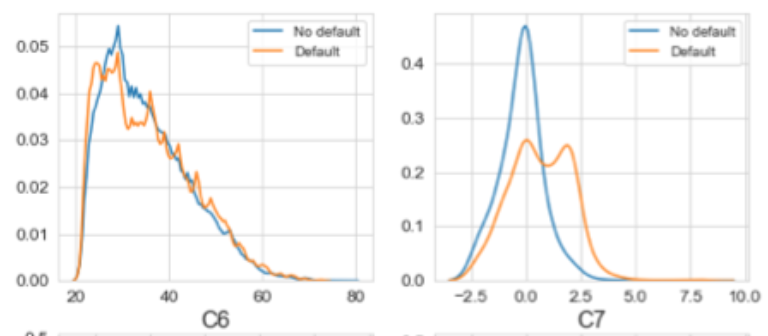
\includegraphics[width=6cm, height=4cm]{figure1.png}
 \caption{Figure 1}
 \label{fig:figure1}
\end{figure}
The first visualisation tool applied was density plots. A density plot visualises the distribution of data over a continuous interval. As shown in the figure below, this process involved grouping the data for each independent variable based on the dependent classes. This process was done for all the independent variables and it was    found that the most representative attributes were \textbf{PAY0}, \textbf{PAY2}, \textbf{PAY3}, \textbf{PAY4}, \textbf{PAY5}, \textbf{PAY6}, \textbf{SEX}, \textbf{EDUCATION}, \textbf{MARRIAGE}. This indicated in the figure below highlighting the density plots for \textbf{PAY0} and \textbf{AGE} with \textbf{AGE} showing significantly less representation than \textbf{PAY0}. \\ \\
\begin{figure}[h]
 \centering
 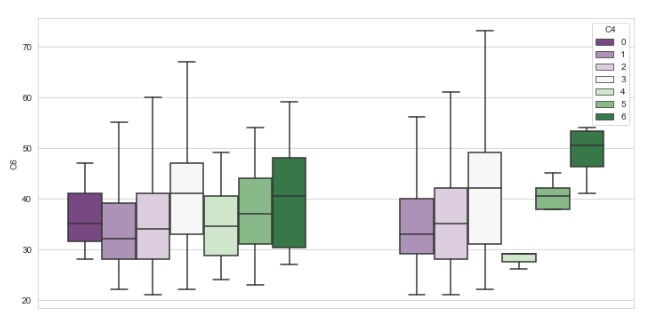
\includegraphics[width=6cm, height=4cm]{figure2.png}
 \caption{Figure 2}
 \label{fig:figure2}
\end{figure}
Box plots are another tool that can be used to help better visualise a dataset. They provide a better way to consider range and other important characteristics regarding the dataset. Figure 2 \ref{fig:figure2}below compares age (x-axis) and default status (y-axis), grouping each box plot based on education status. The box plot distributions for graduate, university and high-school are relatively similar for both default statuses. This indicates that these education groups are not very determinant regarding default. However, this changed when considering the remaining education categories. As figure 2 shows, the box plots for education statuses 4-6 vary significantly for both default statuses. Default status 1 shows little variance indicating more agreement.\\ \\
\begin{figure}[h]
 \centering
 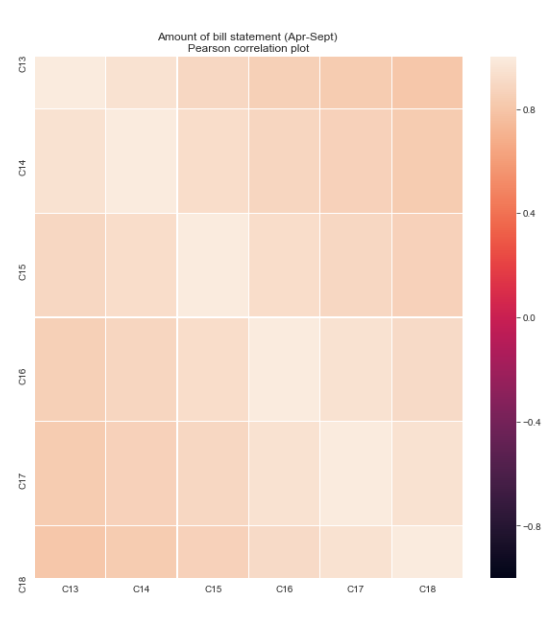
\includegraphics[width=6cm, height=4cm]{figure3.png}
 \caption{Repayment Status}
 \label{fig:figure3}
\end{figure}
A correlation matrix is shown in Figure 3\ref{fig:figure3}. This is a table that shows the value of the correlation coefficient between sets of variables. This correlation matrix compares repayment status and default status. There is some correlation between repayment status and default status. This suggests a link between an ability to keep up with payments and defaulting. Similar matrices were also created for the other independent variables. Some correlation was also found between balance limit and default status whilst not much was found between default status and other categorical variables. This indicates that balance limit could be a crucial factor in determining default status. \\ \\
Ultimately, some patterns can be found, but no clear conclusion can be made with this level of analysis. Therefore, a more in-depth approach is required to successfully predict the default status of customers. 

\subsection{Dimensionality Reduction: Principal Component Analysis (PCA)}
As we can see from the data description, $X12$ to $X17$ are the variables for \textbf{Amount of bill statement}, $X18$ to $X23$ are the variables for \textbf{Amount of previous payment}, also, $X1$ for the \textbf{Amount of given credit}. So there is no doubt that there are correlations between these variables. As such, we can think of this problem as we have k+n vectors in k dimensions. We approach this problem by finding the principal components. Principal components are directions along which original data are highly variable. We can achieve this by projecting each data point $x_n$ onto a scaler unit $u_{1}^{T}x_n$ 

The next thing of interest is, how do we choose the variables after PCA? Fewer variables mean some information will be lost, so a clear strategy would be to keep the variables that contain the most amount of information, in other words, explain most of the variances.
The total variance present is:
\begin{equation}
\frac{1}{N} \sum_{n=1}^{N} x_{n}^{T} x_{n}
\end{equation}
The variance by $k$th principal components is:
\begin{equation}
\frac{1}{N}\sum_{n=1}^{N}(x_{n}^{T}\mu_{k})^{T}(x_{n}^{T}\mu_{k})=\lambda_k
\end{equation}
The proportion of variance explained by $k$th principal components is:
\begin{equation}
\frac{\lambda_k}{\frac{1}{N}\sum_{n=1}^{N}x_{n}^{T}x_{n}}
\end{equation}
In python, we can simply set the parameter in PCA to be 0.95, which select the number of components such that the amount of variance that needs to be explained is greater than the percentage specified by the number of components.
Another thing worth mentioning is that PCA takes into account the scale of variables. Since each variable has different scales, it will not be fair to feed them into PCA directly, so a standardisation is applied before the PCA.


\section{Overview of Methodology}
The fundamental basis of the methodology was to test and compare three uniquely different algorithms, then select the most effective one for use in the final solution. To begin with, the data was explored using h20 and coupled with PCA to gain a better understanding of the underlying variables in the problem. Numerous sources\cite{source1,source2,source3} were consulted for this section to ensure all potential options were considered. Once the data is fully prepared, it is fed into the three different algorithms used: Random Forest, LDA, and Neural Networks. Extensive research\cite{h2o,research2}on the most suitable algorithms was carried out in order to justify the algorithms selected. After the final accuracy scores of each algorithm were successfully obtained, they were cross-referenced against one another with the objective of selecting the final, most effective,  model algorithm.\\

Features Engineering is a key component of any machine learning algorithm, it is essential that a variety of approaches are explored before arriving at a final method. Firstly, correlation matrices and heat maps were considered as a way to display the dependencies of the input variables to the output variables. The correlation coefficients of the independent variables were significantly smaller than anticipated. As a result of this, it was harder to differentiate between which features are most related to the output variable and therefore, to conclude, this method is not viable for the problem at hand. PCA was considered as a viable method of Feature Engineering and was implemented into our final method. \\

Each algorithm was trained and evaluated by splitting the training data into two different subsets. The validation data set was typically 20\% of the training data for the algorithms used. Once the data was split, each model was then fitted using the appropriate predictor and outcome variables (after preprocessing). Additionally, each algorithm was specifically tuned to the data set to optimize the results obtained, these steps will be discussed further in section 4.

\subsection{Key concepts used in the following methods:}
\label{sec:key}
\subsubsection{Pipelines:}
This concept is easily imported from the \textit{sklearn.pipeline} library and it enables the easy manipulation of parameters. This concept was used thoroughly in the LDA, QDA and Logistic Regression models presented further below in the Model training and Validation section.
\subsubsection{GridsearchCV:}
This function is, imported from another \textit{sklearn} library called \textit{sklearn.model\_selection}. Through this function, the model will be continuously looped until all possibilities have been computed and will then return the model with the highest level of accuracy depending on the specified options. In the sections below the \textit{Pipelines} and the \textit{GridsearchCV} will be combined to enable models to be tested with different classification functions and dimensionality reduction methods.

\subsection{Other attempted Methods:}
\subsubsection{Quadratic Discriminant Analysis (QDA)\cite{qda}:}
This function is a classifier with a quadratic decision boundary, which uses \textit{Bayes} rules. It’s function is easily accessible through the use of the \textit{sklearn.qda} library. Furthermore, it is normally considered to be a good model for extremely large data sets however, in our case it was not an optimal scenario. The reasoning behind this is that when a pipeline with such a classification function is used the parameters of a specified dimensionality reduction method are too low. Using PCA as an example, when the pipeline is subjected to the \textit{GridsearchCV} function such the returned \textit{n\_components} would be the lowest possible, which would affect our results as much of the required features will not be included and thus making the model one hard to trust. 
\subsubsection{Logistics Regression:}
Such a model is mostly concerning binary-classification problems, such as this. As mentioned in part 3.2\ref{sec:key}, while performing the \textit{gridsearch} function we attempt to find the best option for the C hyperparameter, while having the solver and \textit{max\_iter} parameter set to \textit{‘lbfgs’} and \textit{‘500’}. This C hyperparameter is known as the inverse regulation parameter, which means that the lower the value the higher the regulation. This is taken from the corresponding Pipeline containing PCA and LR\cite{lr}, \textit{pipe\_pca\_lr}. Once \textit{gridsearch} is complete we gather an accuracy score of the model on the training dataset has value of 80.59\%, with the list of parameters used.
\subsubsection{SelectKBest\cite{SelectKBest}:}
\textbf{SelectKBest}, is another dimensionality reduction method, which uses k highest score as a way of feature selection and is also imported through the library \textit{sklearn.feature\_selection}. The important difference between the two methods is that \textit{selectKbest} uses the k parameter, which is the number of top features to select, which differs from the PCA’s approach of using \textit{n\_components}. 

\section{Model Training and Validation}
As mentioned in the introduction, three different algorithms were trained using the training data and then validated. Their results were cross-referenced with one another and the complexity and reliability of each algorithm were considered when deciding the most effective method.
\subsection{Random Forest (RF):}
The Random Forest (RF) algorithm is purely an amalgamation of various Decision Trees\cite{h2o}, an intuitive model that can be thought of as a series of \textit{yes/no} questions asked about the data.

The preprocessing steps for RF consisted of converting the categorical variables into numeric (using one-hot encoding) so that the numeric significance is understandable to the algorithm. The categorical variables were converted into dummy/indicator variables. Once this was completed, the numeric variables were standardized so that the PCA can be effectively implemented. Finally, the data then underwent PCA. 

After conducting the PCA there is now a total of 88 variables, which consist of the conventional and dummy variables. Specifically to the RF algorithm, further features selection was conducted to view which of these 88 variables have the greatest effect on the outcome variable. A feature importance graph  was generated (Figure: Feature Importance\ref{fig:feature-Importance}), it displays the relative importance of the variables to the outcome variable. This allows further reduction in the dimensionality of the data, as only the highest-scoring variables (above 0.005) were then kept for training the algorithm. The subset consisted of 33 features and decreased the accuracy by only 1.2\%. Thus, for a small cost in accuracy the number of features decreased by approximately 63\%.\\ \\
\begin{figure}[h]
 \centering
 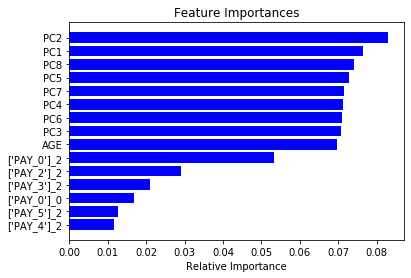
\includegraphics[width=6cm, height=4cm]{feature-importance.png}
 \caption{Feature Importance}
 \label{fig:feature-Importance}
\end{figure}

Hyperparameters were also considered during the training phase to try and optimize the results\cite{rf-result}. Overfitting is a common limiting factor for this algorithm, where the model performs better on the training subset than the validation subset. To reduce this error an optimum maximum depth value was determined using a ROC AUC curve (Figure: ROC AUC\ref{fig:rf-auc}) for the training and testing sets\cite{rf-testing}. The optimum maximum depth, as seen on the graph, was calculated to be 13 for the testing data provided. It’s visible that the model overfits for large depth values and shows stabilization with increasing depth. This optimum value was then incorporated into the final model prediction, showing a slightly improved accuracy score.\\ \\
\begin{figure}[h]
 \centering
 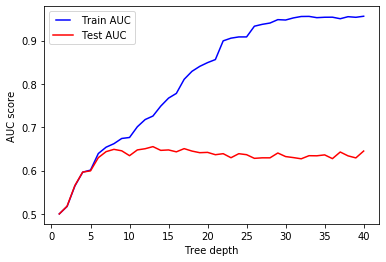
\includegraphics[width=6cm, height=4cm]{rf-auc.png}
 \caption{ROC AUC}
 \label{fig:rf-auc}
\end{figure}

The RF algorithm was then trained by splitting the data into random training and validation subsets against the predictor variables and outcome variables. The size of the testing data was set as 20\% of the data frame. The random state seed was kept constant at a value of 5. Both the hyperparameter optimization and further feature selection were incorporated into the final method. 

\subsection{Linear Discriminant Analysis (LDA):}
Linear Discriminant Analysis, known more simply as LDA\cite{lda}, is a classification algorithm, which is performed in relative simplicity during both the preparation and application of the model. For our model, LDA is imported from the \textit{slearn.discriminant\_analysis} library. \\

It is important to not that when LDA\cite{sci-lda} is performed it makes 2 key assumptions about your data. Firstly, it assumes the data has a Gaussian nature and it also assumes each variable to have identical mean. Both of these assumptions are used to enable the model to predict a mean and variance for each class of the data. \\

In preparation of its implementation the data is required to undergo transformation and exploration, with the use of PCA as a dimensionality reduction method, as mentioned above. Moreover, to achieve the best possible model with PCA the use of the \textit{GridsearchCV()} (referred to as \textit{gridsearch} in this paper) function. Furthermore, the parameters of the chosen model can also be displayed through \textit{gs\_pca\_lda.best\_params\_} in the notebook, where \textit{gs\_pca\_lda} is the name given to this specific gridsearch function. The function can also be used to predict the best parameters for the specific classification model, such as one containing LR, however, due to the set parameters of the LDA such an addition is not necessary. 

\begin{figure}[h]
 \centering
 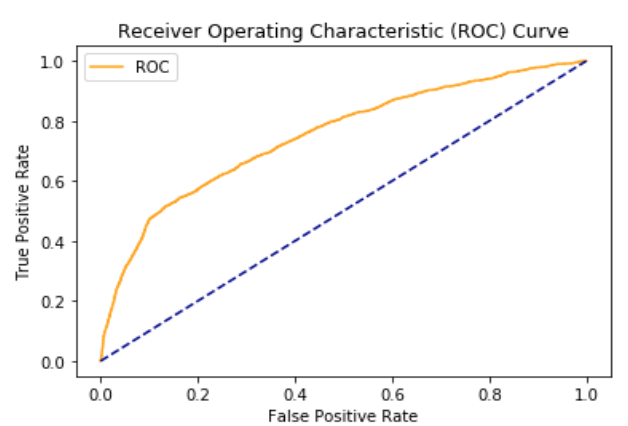
\includegraphics[width=6cm, height=4cm]{lda-roc.png}
 \caption{ROC curve for LDA with PCA}
\end{figure}
							
LDA has 2 specific parameters that remain unchanged throughout the model. The first parameter is the solver, while the second is named shrinkage, which is a tool used to improve the covariance matrix estimation. From \textit{pipe\_pca\_lda}, which is the pipeline containing PCA and LDA, the parameters are seen to have the values of ‘eigen’ and ‘auto’. The \textit{‘eigen’} solver is one that permits the use of the shrinkage parameter and performs Eigenvalue Decomposition, while the ‘auto’ value is simply performing an automatic shrinkage of the data. From the notebook we can see that once the \textit{gridsearch} is performed the accuracy score of the model on the training dataset has value of 80.4\%

It is also important to note that LDA was not only conducted with the PCA approach for dimensionality reduction however, SelectKBest, which is defined in the Methodology overview, was also attempted. Similarly to the PCA with LDA model described above, a pipeline, named \textit{pipe\_skb\_lda}, was created. Another \textit{gridsearch}, named \textit{gs\_skb\_lda}, is created to find the optimal value of k, with the LDA to achieve the best possible accuracy. The returned accuracy is 81.62\%, which is slightly higher than the PCA’s approach. 

\subsection{Neural Networks:}
Among so many architecture of neural networks, FFN (Feedforward neural network) is chosen. The reason for choosing FFN over RNN is the dataset in hand is a combination of categorical and numeric data, and data of time series is missing, we don’t need RNN to exhibit it’s dynamic behavior. \\ \\

Before we build our model, input data are treated as different feature columns. Firstly initialize an empty list to store the features we want to feed into our model. The numeric columns are identified as ‘numerics’ by using \textit{feature\_column.numeric\_column()} in \textit{tensorflow} package. \\ \\
But we take extra cautions when dealing with categorical variables. If we simply transform the categorical variables into numerics using one-hot encoding, a lot of information will be lost. For example, In the \textbf{EDUCATION} sector, we have 1 to 4 representing graduate school, university, high school and others. Clearly the gap between graduate students and high school students is much larger than the gap between graduate students and university students, but one hot encoding miss these information as there will only be \textit{‘0’} or \textit{‘1’} indicating whether the person is within a particular category. The technique adopted here to keep the information is ‘embedding’\cite{embedding}. Firstly we convert the categorical variables into dummy variables by using one-hot encoding, which generates a $m \times n$ matrix (m for the number of observations and n for the number of different categories), we simply multiply this new generated matrix by another $n \times k$ (n for the number of different categories, k for the number of target categories) embedding matrix, this embedding matrix is like the weighting matrices between layers, but instead of staying between the layers, it is before the input layer. Usually we don’t allow the neural network to make changes to our input layer, but this time we allow it to train the parameters in embedding matrix during optimization procedure. The one-hot encoding is implemented by 
\textit{feature\_coulumn.categorical\_column\_with\_identity} and embedding is implemented by  \textit{feature\_column.embedding\_column} in \textit{tensorflow} package.\\ \\

After the feature columns are constructed, we can build our model. All the layers including input layer are treated as dense feature layer, since we are using a FFN model. We start our initial attempt by feeding in our data with batch size of 64, 2 hidden layers. Sigmoid function is selected as the activation function for output with no doubt. 
\begin{equation}
f(X_i)=\frac{1}{1+e^{-X_i}}
\end{equation}  and the graph of sigmoid function is:
\begin{figure}[h]
 \centering
 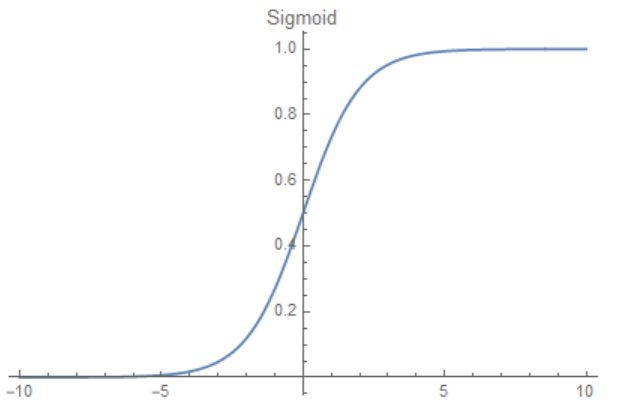
\includegraphics[width=6cm, height=4cm]{sigmoid.png}
 \caption{Sigmoid function}
\end{figure}

We can see one important feature of this function is that the high value will have the high probability but not the higher probability. This is the ideal feature for binary classification in logistic regression model. We chose this activation function as our output is binary.

For the activation function between hidden layers, we have two choices. One is Softmax function: 
\begin{equation}
f(X_i)=\frac{e^{X_i}}{\sum_{j=0}^{k}e^{X_j}}
\end{equation}
The graph of softmax function is:
\begin{figure}[h]
 \centering
 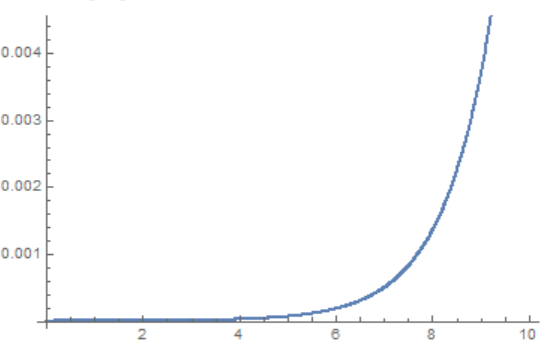
\includegraphics[width=6cm, height=4cm]{softmax.png}
 \caption{Softmax function}
\end{figure}

One important property of this function is that the high value will have a higher probability than other values. Since we don’t want to simply throw away some properties if the importance seem to be low, instead we give shrink the perceptron with a certain amount. 
Another function is Rectifier. The formula is very simple:
\begin{equation}
f(x)=max(0,x)
\end{equation}
 The graph takes the shape:
 \begin{figure}[h]
 \centering
 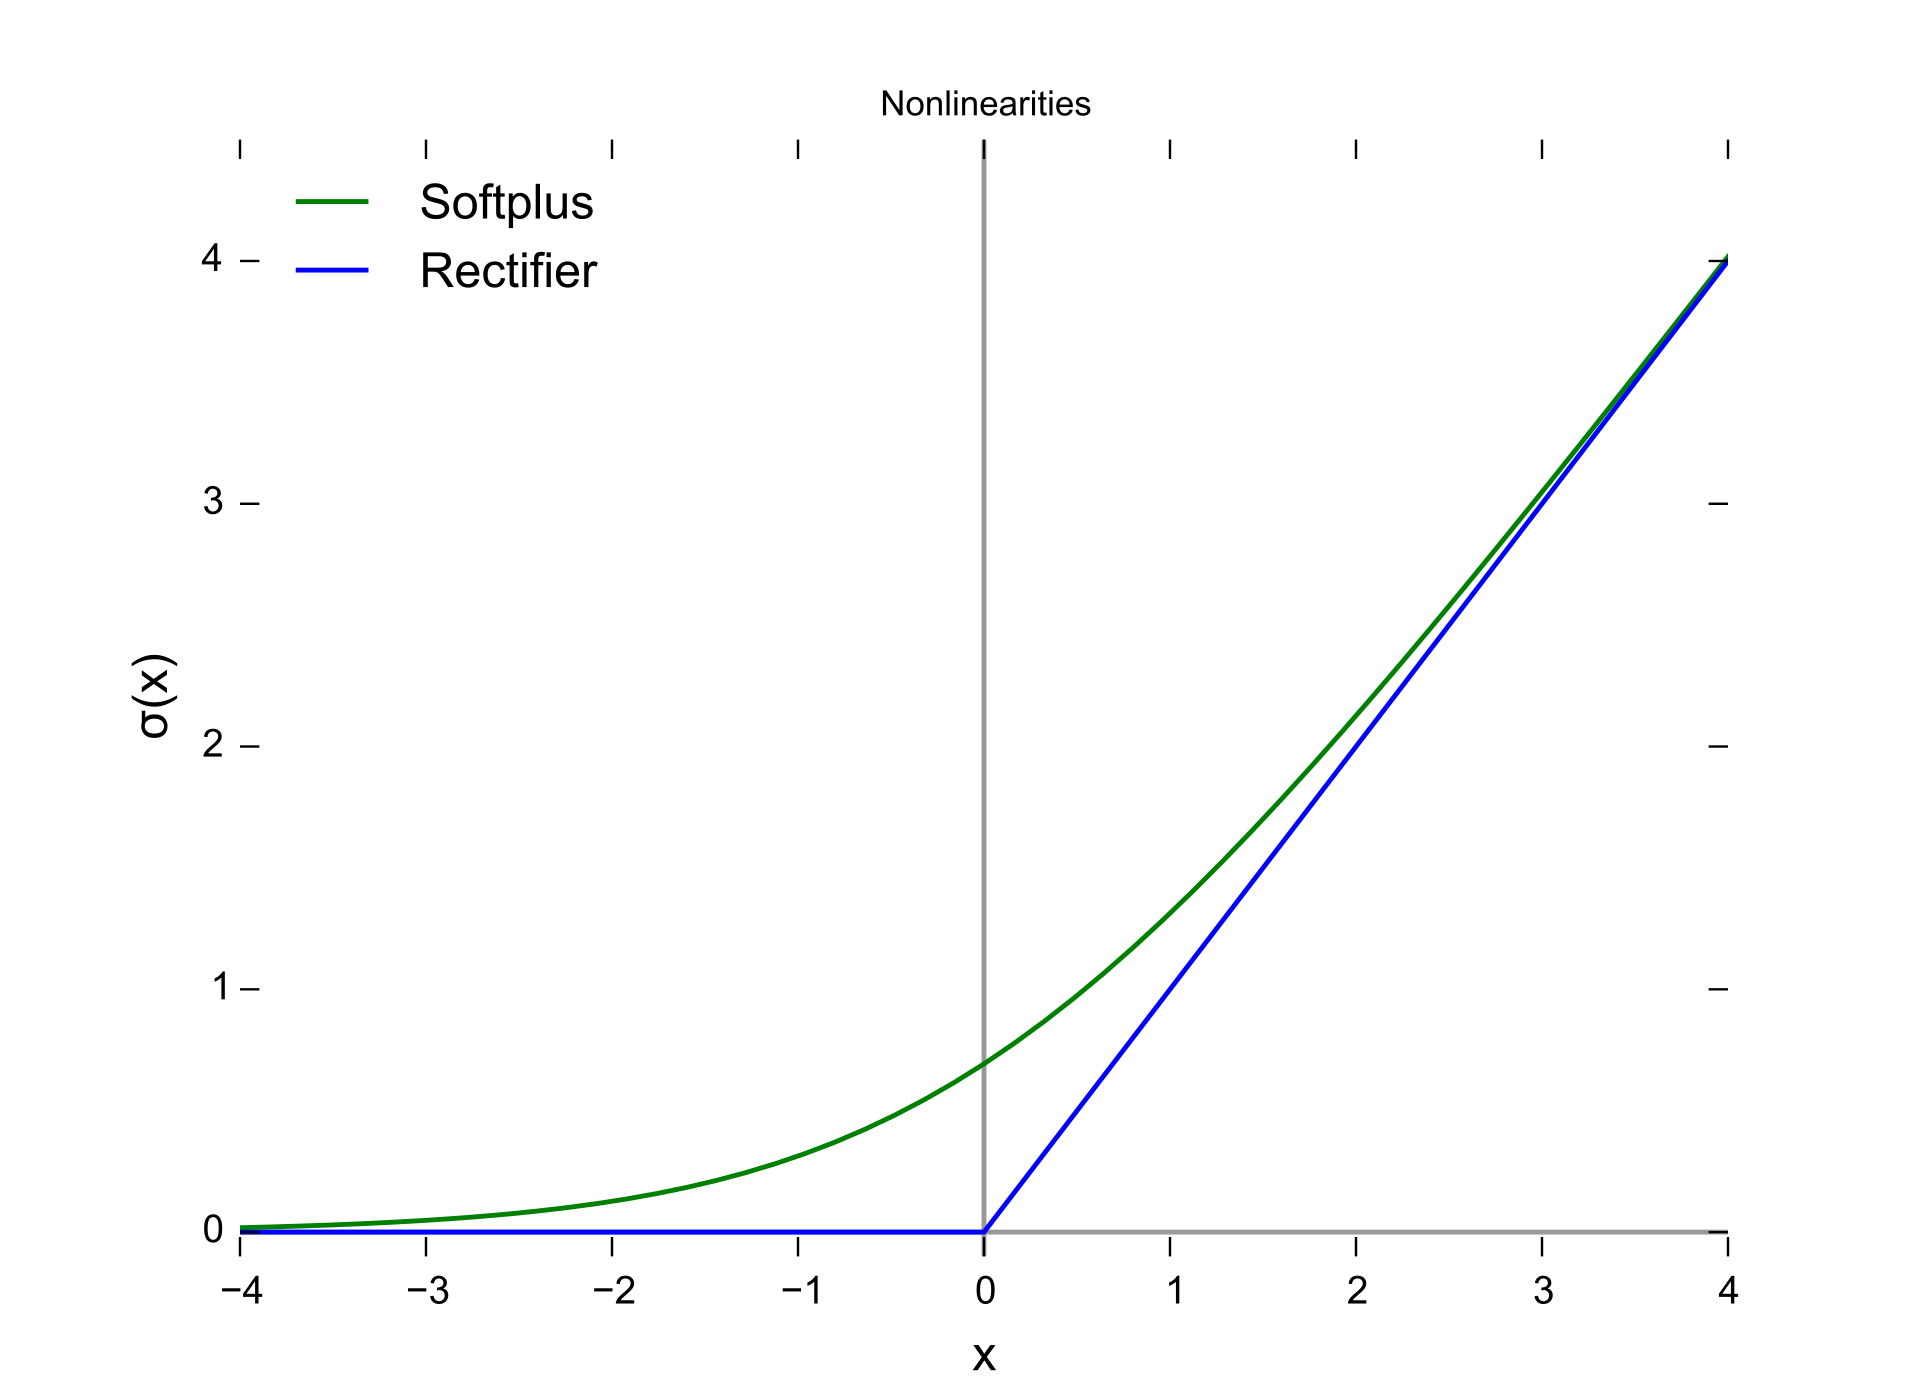
\includegraphics[width=6cm, height=4cm]{relu.png}
 \caption{Relu function}
\end{figure}

This function is similar to Softmax function, but a linear growth in probability is applied as the variable becomes larger.

Stochastic gradient descent is chosen as the optimizer, number of epochs are chosen to be 10 at first, but we notice the validation accuracy starts to fall after 3 epochs, so we terminate the training at 3 epochs. 

The first attempt gives us a prediction score of 0.789. So we tried the following steps to make the model work more efficiently:
'AGE' will be transformed into bucket variable, since it makes more sense to treat them like people of different age groups.
Try to standardize the numeric variables.
Do a PCA to the numerics and see if we can throw away some variables.

Besides the above methods, we also tune the parameters. An extra layer with Relu activation function is added to the model, a new optimizer Adam is chosen instead of SGD we used in the previous model. Adam can be looked at as a combination of RMSprop and Stochastic Gradient Descent with momentum. It uses the squared gradients to scale the learning rate like RMSprop and it takes advantage of momentum by using moving average of the gradient instead of gradient itself like SGD with momentum\cite{adam} .This optimizer is available in Keras\cite{optimizer}.

For this time, the validation accuracy starts to decrease after 5 epochs, so we terminate the training process there.


\section{Model Results:}
Each algorithm was trained and validated using the training data provided. The final accuracy of each model was recorded and cross-referenced with one another, the results are presented in Table 1.
\begin{table}[h]
\centering
\begin{tabular}{ |p{3cm}|p{3cm}|p{3cm}|p{3cm}|  }
 \hline
 &Random Forest (RF)&Linear Discriminant Analysis (LDA)&Neural Networks (NN)\\
 \hline
 Accuracy on training data (\%) & 82.40 & 80.40 & 83.25\\
 \hline
\end{tabular}
\caption{Algorithm accuracy scores}
\end{table}
The algorithms will be compared in terms of their complexity, reliability, and workload. To begin with, the RF model is by far the simplest out of the three, with it only requiring 4 features to obtain an accuracy of 82.40\%. Both NN and LDA contained far more features than RF and are fundamentally more complex by nature. However, NN still produces a more accurate result than RF. \\ \\

The reliability of each algorithm depends upon the data that it is processing and its limitations. The testing data provided is tabular, which all three algorithms can process well to a certain degree. The NN approach tends to be more reliable than the others due to its ability to generalize. After learning from the preliminary data inputs and the relationships, it can then deduce hidden relationships on unseen data as well, thus making the model generalize and predict on unseen data. This ultimately increases the reliability of the NN algorithm compared to RF and LDA. RF’s accuracy plateaus relatively early when feeding it new data after a certain amount. Whilst NN continues to improve its accuracy, providing increasingly reliable results. Regarding LDA, the algorithm suffers from multicollinearity, which will negatively affect the algorithms results. Multicollinearity generally occurs when there are relatively high correlations between multiple predictor variables, which there are for the data set provided. This limitation will reduce the model’s reliability.\\ \\

It should be clear that the NN algorithm has the greatest workload out of the three. The data preprocessing section for NN is very time-consuming compared to LDA and RF. NN requires filling of missing data points and converting categorical data into numerical. Additionally, NN needs feature scaling too. If features aren’t scaled into the same ranges then features that have greater values will be considered as more important when training the model, which is not desired. The preprocessing sections of RF and LDA are far simpler and less time-consuming than NN. For RF you solely need to ensure there are no missing values within your data and also convert categorical data into numerical. Of course, there are additional preprocessing steps that can be conducted but they are not compulsory.\\ \\
 
In conclusion, the NN model seems to produce the most accurate and reliable results on the testing data set and will be used for the final predictions. Considering the complexity of this model relative to RF and LDA, it is worthwhile to implement due to it being a more heavily robust algorithm.

\section{Final Predictions on Testing Data}
As mentioned in the previous section, the Neural Network approach (NN) has been selected for the final predictions on the testing data. The preprocessing sections and tuning for the classifier have remained the same as before and can be viewed in the jupyter notebook.

The final NN algorithm produced an accuracy score of 83.25\% on the testing data. The implications of this value is that using the model developed, it is possible to predict with 83.25\% accuracy that a customer is likely to default next month. The NN algorithm does not indicate which of the predictor variables have the greatest significance towards whether or not someone will default. 


\section{Conclusions}
To begin with,  it's worthwhile to mention that there is a wide range of potential methods to approach this problem.  As shown within this paper, different approaches with varying complexity can still produce similar results. This is primarily due to the fact that the data of the problem is not incredibly complex. Therefore, the different algorithms can make predictions of a relatively high degree of accuracy. 

The final approach implemented (NN) made predictions of a substantially high degree of accuracy. However, when comparing the three approaches (RF, LDA and NN)  there isn't that much of a significant variation between their accuracies. Even though they vary in sophistication and complexity, the difference between the highest and lowest accuracy scores is only 2.85\% (NN \& LDA). Yet the intricacy of the NN model is far greater and more sophisticated than that of LDA. 

A potential possibility for future attempts at this project is to try and implement a larger number of unique high level algorithmic approaches. This would prove to be an intriguing proposition, to see how different sophisticated algorithms model and predict the data. Essentially, it would demonstrate whether you can obtain a larger variation between the accuracies of different algorithms. 


\bibliographystyle{unsrt}  

\begin{thebibliography}{1}

\bibitem{h2o}
Will Koehrsen.
\newblock\href{https://towardsdatascience.com/an-implementation-and-explanation-of-the-random-forest-in-python-77bf308a9b76}{ An Implementation and Explanation of the Random Forest in Python.}

\bibitem{source1}
Abhini Shetye.
\newblock\href{https://towardsdatascience.com/feature-selection-with-pandas-e3690ad8504b}{Feature Selection with Sklearn and Pandas}

\bibitem{source2}
Sayak Paul.
\newblock\href{https://www.datacamp.com/community/tutorials/feature-selection-python}{Feature Selection in Python}

\bibitem{source3}
Matt Brems.
\newblock\href{https://towardsdatascience.com/a-one-stop-shop-for-principal-component-analysis-5582fb7e0a9c}{A One-Stop Shop for Principal Component Analysis}

\bibitem{research2}
James Le.
\newblock\href{https://www.codementor.io/@james_aka_yale/a-gentle-introduction-to-neural-networks-for-machine-learning-hkijvz7lp}{A Gentle Introduction to Neural Networks for Machine Learning}

\bibitem{lr}
Sklearn.
\newblock\href{https://scikit-learn.org/stable/modules/generated/sklearn.linear_model.LogisticRegression.html}{Skelearn Documentation for logistic regression}

\bibitem{qda}
Sklearn.
\newblock\href{https://scikit-learn.org/0.16/modules/generated/sklearn.qda.QDA.html}{Sklearn Documentation for QDA}

\bibitem{SelectKBest}
Sklearn.
\newblock\href{https://scikit-learn.org/stable/modules/generated/sklearn.feature_selection.SelectKBest.html}{Sklearn Documentation for Select K Best}

\bibitem{rf-result}
Sklearn.
\newblock\href{https://scikit-learn.org/stable/auto_examples/tree/plot_tree_regression.html}{Sklearn Documentation for Decision Tree}

\bibitem{rf-testing}
Reilly Meinert.
\newblock\href{https://towardsdatascience.com/optimizing-hyperparameters-in-random-forest-classification-ec7741f9d3f6}{Optimizing Hyperparameters in Random Forest Classification}

\bibitem{lda}
Jason Brownlee.
\newblock\href{https://machinelearningmastery.com/linear-discriminant-analysis-for-machine-learning/}{Linear Discriminant Analysis for Machine Learning}

\bibitem{sci-lda}
Sklearn.
\newblock\href{https://scikit-learn.org/stable/modules/generated/sklearn.discriminant_analysis.LinearDiscriminantAnalysis.html}{Sklearn documentation for LDA}

\bibitem{embedding}
Deepak Mishra.
\newblock\href{https://towardsdatascience.com/categorical-embedding-and-transfer-learning-dd3c4af6345d}{Categorical Embedding and Transfer Learning}

\bibitem{adam}
Vitaly Bushaev.
\newblock\href{https://towardsdatascience.com/adam-latest-trends-in-deep-learning-optimization-6be9a291375c}{Adam — latest trends in deep learning optimization.
}

\bibitem{optimizer}
Keras.
\newblock\href{https://keras.io/optimizers/}{Keras documentation for optimizers}


\end{thebibliography}

\end{document}
    